% Options for packages loaded elsewhere
\PassOptionsToPackage{unicode}{hyperref}
\PassOptionsToPackage{hyphens}{url}
%
\documentclass[
  11pt,
]{article}
\usepackage{amsmath,amssymb}
\usepackage{lmodern}
\usepackage{ifxetex,ifluatex}
\ifnum 0\ifxetex 1\fi\ifluatex 1\fi=0 % if pdftex
  \usepackage[T1]{fontenc}
  \usepackage[utf8]{inputenc}
  \usepackage{textcomp} % provide euro and other symbols
\else % if luatex or xetex
  \usepackage{unicode-math}
  \defaultfontfeatures{Scale=MatchLowercase}
  \defaultfontfeatures[\rmfamily]{Ligatures=TeX,Scale=1}
\fi
% Use upquote if available, for straight quotes in verbatim environments
\IfFileExists{upquote.sty}{\usepackage{upquote}}{}
\IfFileExists{microtype.sty}{% use microtype if available
  \usepackage[]{microtype}
  \UseMicrotypeSet[protrusion]{basicmath} % disable protrusion for tt fonts
}{}
\makeatletter
\@ifundefined{KOMAClassName}{% if non-KOMA class
  \IfFileExists{parskip.sty}{%
    \usepackage{parskip}
  }{% else
    \setlength{\parindent}{0pt}
    \setlength{\parskip}{6pt plus 2pt minus 1pt}}
}{% if KOMA class
  \KOMAoptions{parskip=half}}
\makeatother
\usepackage{xcolor}
\IfFileExists{xurl.sty}{\usepackage{xurl}}{} % add URL line breaks if available
\IfFileExists{bookmark.sty}{\usepackage{bookmark}}{\usepackage{hyperref}}
\hypersetup{
  pdftitle={How did the second Covid-19 lockdown in Denmark affect tobacco purchases among frequent smokers?},
  hidelinks,
  pdfcreator={LaTeX via pandoc}}
\urlstyle{same} % disable monospaced font for URLs
\usepackage[margin=3cm]{geometry}
\usepackage{graphicx}
\makeatletter
\def\maxwidth{\ifdim\Gin@nat@width>\linewidth\linewidth\else\Gin@nat@width\fi}
\def\maxheight{\ifdim\Gin@nat@height>\textheight\textheight\else\Gin@nat@height\fi}
\makeatother
% Scale images if necessary, so that they will not overflow the page
% margins by default, and it is still possible to overwrite the defaults
% using explicit options in \includegraphics[width, height, ...]{}
\setkeys{Gin}{width=\maxwidth,height=\maxheight,keepaspectratio}
% Set default figure placement to htbp
\makeatletter
\def\fps@figure{htbp}
\makeatother
\setlength{\emergencystretch}{3em} % prevent overfull lines
\providecommand{\tightlist}{%
  \setlength{\itemsep}{0pt}\setlength{\parskip}{0pt}}
\setcounter{secnumdepth}{-\maxdimen} % remove section numbering
\newcommand*{\secref}[1]{Section~\ref{#1}}
\usepackage{xcolor,colortbl}
\definecolor{gray1}{gray}{0.9}
\ifluatex
  \usepackage{selnolig}  % disable illegal ligatures
\fi

\title{How did the second Covid-19 lockdown in Denmark affect tobacco
purchases among frequent smokers?}
\usepackage{etoolbox}
\makeatletter
\providecommand{\subtitle}[1]{% add subtitle to \maketitle
  \apptocmd{\@title}{\par {\large #1 \par}}{}{}
}
\makeatother
\subtitle{A study analysing tobacco habits based on a time series of
electronic receipts from various Danish supermarkets.}
\author{}
\date{\vspace{-2.5em}\small 06 September 2021}

\begin{document}
\maketitle

\hypertarget{introduction}{%
\section{Introduction}\label{introduction}}

It is well-known that smoking is a risk factor for different diseases,
cardiovascular disease amongst others \cite{fda}. 73 \% of smokers in
Denmark wish to quit, still, the smoking prevalence among adults in
Denmark is \(17 \%\) \cite{sundhedsstyrelsen}. A pandemic is a radical
societal intervention that affects the everyday life of people around
the world, and the effect of the early phase of the COVID-19 pandemic on
smoking cessation has been investigated in several countries. A Turkish
study found that the COVID-19 outbreak was effective on smoking
cessation \cite{turkish}, while the Wave 3 (2020) ITC Four Country
Smoking and Vaping Survey including 6870 smokers conducted in Australia,
Canada, England and the US showed that overall nearly \(50 \%\) of the
smokers thought about quitting, but only \(14 \%\) actually made a quit
attempt \cite{wave3}. The thoughts of quitting have been related to the
fear of COVID-19, justified by increasing evidence that smoking results
in a graver COVID-19 disease progression \cite{unionbrief}. So, the
pandemic might offer a ``leanable window'' \cite{todolist} or a
``teachable moment'' as they phrase it in \cite{addiction}, for smokers
to change their behaviour. Therefore, understanding these behavioural
changes due to the pandemic is important to obtain more focused and
targeted interventions on smoking cessation. \newline Conversely, the
pandemic also resulted in increased stress levels, as national lockdowns
led to a series of restrictions being put into place, including closed
schools and restaurants, physical distancing measures and remote
workplaces. Many smokers report smoking as a way to cope with high
levels of stress, and a recent study associated the initial COVID-19
lockdown in California with an increased cigarette consumption among
current smokers \cite{california}. A possible cause mentioned was an
increased opportunity for smoking due to virtuel workplaces not being
protected by indoor smokefree workplace laws, which underlines the
importance of protective policies. Thus, understanding the public health
effect of the COVID-19 pandemic and identifying exposed groups are
important for developing and focusing targets for intervention. This is
underlined in \cite{UK_inequalities}, where they conclude that there are
socio-economic disparities in the association between smoking and
COVID-19 infection based on a study of 53000 adults in the UK. In
conclusion, there are conflicting results from various countries about
how the early phase of the COVID-19 pandemic affected smoking cessation,
and in all studies reviewed, the authors inform about limitations and
possible improvements about the study design that one should be aware of
when interpreting the results. In this paper, we suggest a novel
approach by using a time series of credit card transactions from 8800
subjects obtained in the period July 2018 to August 2021 from a large
number of Danish supermarkets.

\hypertarget{a-novel-approach-tracking-smoking-behaviour-over-time-using-credit-card-transactions}{%
\subsection{A novel approach: Tracking smoking behaviour over time using
credit card
transactions}\label{a-novel-approach-tracking-smoking-behaviour-over-time-using-credit-card-transactions}}

To date, all existing literature concerning this topic, as described
above, is based on questionnaires about smoking behaviour and thoughts
about smoking and COVID-19. Common for these is that the questions are
asked at one (or more) specific point in time, which does not allow for
accurate tracking of changes over time \cite{UK_inequalities}. During
the pandemic, things changed so rapidly, that daily (even hourly) data
is better suited to capture an accurate development, which the credit
card transactions represent. This longitudinal data also gives the
opportunity to investigate whether or not people actually return to
their old habits again as time passes. A study using a similar type of
data examined trends in the number of visitors, followers, and
subscribers on smoking cessation digital platforms from January to April
2020, and compared these traffic data to a control period
\cite{digital}. Here, they concluded that the initial increase in the
number of visitors and subscribers was followed by a decline in traffic,
and investigation of such trends is also possible using our credit card
transaction data. \newline Secondly, we avoid recall bias and
self-reported bias, which all existing studies suffer from to some
degree. Only a few of the studies are based on real time data collection
(before and after a COVID-19 lockdown) \cite{california, addiction},
where the latter did not collect data in March 2020, and then changed
from physical to phone interviews. In other studies, data about smoking
habits before lockdown was collected retrospectively after lockdown,
which induces a noticeable recall bias which might affect the results
\cite{UK_inequalities, turkish}. Finally, we conduct our study in a
Danish setting considering recent data from the second wave (lockdown in
Denmark in January 2021-May 2021) which has not been seen yet in the
literature. Limitations about our study design will be included in the
discussion.

\hypertarget{supermarket-transaction-data-structure}{%
\section{Supermarket transaction data
structure}\label{supermarket-transaction-data-structure}}

We have a large amount of supermarket transaction data, where each
transaction is uniquely defined by person and time, and contains at
least one item. In this framework, one can think of a transaction as a
receipt. We let \(K\) denote the total number of transactions in the
database. Letting \(M\) be the total number of items in the database, we
define the set of items to be

\begin{equation}
\label{item_set}
\mathcal{I} = \{I_1, I_2,...,I_M\},
\end{equation}

where item \(m\) is denoted \(I_m\). Each item is associated with a
positive item price and item quantity. This information is contained in
the variables \textbf{item}, \textbf{itemprice} (in DKK) and
\textbf{quantity} as seen in table \ref{trans_table} below. Here, the
gray and white colors mark the different transactions, which are
identified uniquely by a transaction id, \textbf{TID}. Thus, in below
example in table \ref{trans_table}, we have a database consisting of
\(K=5\) transactions, and \(M=9\) items: \[
\mathcal{I} = \{I_1,...,I_9\} = \{bread, dip, dressings, fresh \  eggs, apples, milk, wine, beef, yoghurt\}
\]

Note that the total price of the transaction (\textbf{transactionprice})
is based on itemprice and quantity.

\begin{center}
\begin{table}[h]
\begin{tabular}{|l|l|l|l|r|r|r|} 
\hline
 TID & person & time & item & itemprice & quantity & transactionprice \\
\hline
\hline
\rowcolor{gray1} 1 & 1 & 17-03-2019 08:03:00 & bread & $11.95$ & $1$ & $76.95$\\
\rowcolor{gray1} 1 & 1 & 17-03-2019 08:03:00 & dip & $6.00$ & $2$ & $76.95$\\
\rowcolor{gray1} 1 & 1 & 17-03-2019 08:03:00 & dressings & $53.00$ & $1$ & $76.95$\\
2 & 1 & 19-03-2019 10:15:53 & fresh eggs & $27.95$ & $1$ & $78.40$\\
2 & 1 & 19-03-2019 10:15:53 & apples & $15.00$ & $0.700$ & $78.40$\\
2 & 1 & 19-03-2019 10:15:53 & dip & $10.00$ & $2$ & $78.40$\\
2 & 1 & 19-03-2019 10:15:53 & bread & $19.95$ & $1$ & $78.40$\\
\rowcolor{gray1} 3 & 2 & 02-02-2020 19:34:01 & milk & $9.95$ & $1$ & $9.95$\\
4 & 2 & 14-02-2020 15:55:04 & wine & $109.00$ & $3$ & $479.80$\\
4 & 2 & 14-02-2020 15:55:04 & beef & $49.95$ & $2$ & $479.80$\\
4 & 2 & 14-02-2020 15:55:04 & yoghurt & $18.95$ & $1$ & $479.80$\\
4 & 2 & 14-02-2020 15:55:04 & bread & $5.00$ & $5$ & $479.80$\\
4 & 2 & 14-02-2020 15:55:04 & milk & $8.95$ & $1$ & $479.80$\\
\rowcolor{gray1} 5 & 2 & 20-02-2020 20:24:10 & apples & 2.00 & 2 & $19.00$\\
\rowcolor{gray1} 5 & 2 & 20-02-2020 20:24:10 & bread & 15.00 & 1 & $19.00$\\
... & ... & ... & ... & ... & ... \\
\hline
\end{tabular}
\caption{Transaction data example with 5 transactions and 9 different items.}
\label{trans_table}
\end{table}
\end{center}

\begin{itemize}
\tightlist
\item
  The structure of the transaction data is quite complex: each
  individual has multiple observations of transactions over time, and
  the transactions are quite irregular, meaning that the frequency of
  transactions differs over the weeks, months and between individuals.
\item
  The number of items for each transaction will also vary between
  individuals and through time, as seen in above table. Furthermore, we
  will have new individuals entering the study and people dropping out,
  or even individuals dropping out and entering again, which creates
  missing time gaps.
\item
  To describe this complex data structure we will adapt the theory of
  marked point processes \cite{kar} \cite{last}.
\end{itemize}

\hypertarget{supermarket-transaction-data-a-marked-point-process}{%
\section{Supermarket transaction data: a marked point
process}\label{supermarket-transaction-data-a-marked-point-process}}

\begin{itemize}
\tightlist
\item
  Let \(T_k\) be the time for the \(k^{th}\) supermarket grocery
  transaction. For each transaction time, \(T_k\), one or more items are
  purchased.
\item
  For each transaction time \(T_k\), we have information about the items
  in the transaction, which is described by
  \((X_{1}(T_k),...,X_{M}(T_k))\). Specifically,
  \(X_{m}(T_k)=(P_{m}(T_k), Q_{m}(T_k))\) denotes a vector that contain
  information about price and quantity for item \(m\) at time \(T_k\).
\item
  Consider the first transaction, \(k=1\), from the example in table
  \ref{trans_table}. We have three different items \(I_1=bread\),
  \(I_2=dip\) and \(I_3=dressings\), with corresponding price and
  quantity. For bread we have:
\end{itemize}

\[
X_1(T_1) = (P_1(T_1), Q_1(T_1))=(11.95,1) \in \mathcal{X}_1 = \mathbb{R}^+ \times \mathbb{R}^+
\]

\begin{itemize}
\tightlist
\item
  Thus, for each transaction we have a positive real price and quantity
  for each item. We thus have a \textbf{mark space} for item \(m\) given
  by \(\mathcal{X}_m = \mathbb{R}^+ \times \mathbb{R}^+\).
\item
  With this example in mind, we can now define the marked point process,
  \(\phi\) for the transaction times, \(T_k\).
\end{itemize}

\begin{equation}
\label{point}
\phi = (T_k, (X_1(T_k),...,X_M(T_k)))_{k\geq1}
\end{equation}

where each item has an associated mark space, such that
\(X_1(T_k) \in \mathcal{X}_1,...,X_M(T_k) \in \mathcal{X}_M\). Note that
the mark spaces do not depend on transaction, but only on item, and the
mark space for the entire set of items \(\mathcal{I}\) is given by
\(\mathcal{X}_1 \times...\times \mathcal{X}_M\).

\begin{itemize}
\tightlist
\item
  Note that in most cases the quantities will be natural numbers,
  however, in some cases the quantity will be measured in kg or g, and
  the corresponding price will then be price per kg or price per g. As
  an example, see transaction two in table \ref{trans_table}, where the
  costumer bought 0.7 kg apples that cost 15.00 DKK per kg.
\item
  The defined marked point process from (\ref{point}) counts the number
  of transactions made up to and including time t. When considering the
  process as a function of \(t\), we have an integer-valued step
  function with jumps of size \(+1\), which we assume to be
  right-continous, so that \(N(t)\) is the number of events in the time
  interval \([0,t]\):
\end{itemize}

\begin{equation}
\label{count}
N(t)=\sum_{k\geq 1} I \{T_{k} \leq t\},
\end{equation}

where we assume \(N(0)=0\). See figure below for an illustration of the
marked point process as a counting process \cite{pis}.

\begin{center}
\begin{figure}
\label{point_process}
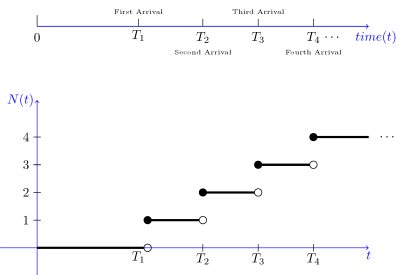
\includegraphics[]{point_process}
\end{figure}
\end{center}

\hypertarget{target-parameter-including-examples}{%
\section{Target parameter including
examples}\label{target-parameter-including-examples}}

\textbf{General target parameter}

\begin{itemize}
\tightlist
\item
  We focus on a fixed time period \(t \in [a,b]\) which is the same for
  every person and an item or itemset \(m^*\). Note that \(m^*\) can be
  a specific item (example \(m^*=\text{tobacco}\)) or an itemset
  (example
  \(m^*=\text{sugary drinks} = \{\text{soda with sugar, ice tea, alcohol free beer}\}\)).
\item
  We now wish to define a target parameter in a general way, such that
  this can be used to investigate different questions. Following
  Appendix 4 (example A4.4 in Last and Brandt), we can write the target
  for \(m^*\) in the time period \([a,b]\) as a Lebesgue-Steiltjes
  integral. Here, we integrate with respect to the counting process
  defined above, as this process marks the arrivals of the transactions.
  We define:
\end{itemize}

\begin{align*}
\mu^{m^*}(a, b) &= E(\int_a^b f(X(t)) dN(t))\\ 
&= \sum_{k: \ a \leq T_k \leq b} E(f(X(T_k))),
\end{align*}

where \(f(X(t))\) is a function defining the nature of the target. See
below two examples for an understanding of this parameter.

\textbf{Example 1}

\begin{itemize}
\tightlist
\item
  We wish to investigate \textbf{the expected number of transactions
  containing} \(m^*\) \textbf{for} \(t\in[a,b]\). Then we would define
  \(f(X(t)) = I_{\{Q^{m^*}(t) > 0, \ P^{m^*}(t) > 0 \}}\). So,
  \(f(X(t))\) denotes the transactions where \(m^*\) was bought, ie. we
  have a positive quantity and price for \(m^*\). From this, we could
  also calculate for example the expected number of daily or monthly
  transactions in the period.
\end{itemize}

\textbf{Example 2 (maybe change notation here)}

\begin{itemize}
\tightlist
\item
  The idea is to estimate the \textbf{expected relative budget spent per
  transaction on} \(m^*\) \textbf{for} \(t\in[a,b]\).
\item
  We use the same expression for \(\mu^{m^*}(a,b)\), however, now
  defining
  \(f(X(t)) = \frac{P^{m^*}(t) \cdot Q^{m^*}(t)}{\sum_{m=1}^M P^m(t) \cdot Q^m(t)}\).
  We would then need to calculate:
\end{itemize}

\[
\mu_{rel}^{m^*}(a,b)= \frac{\mu^{m^*}(a, b)}{\sum_{k=1}^K I_{\{a \leq T_k \leq b \}}},
\]

where the denominater is the number of transactions in the period
\([a,b]\).

\hypertarget{including-covariates-and-grocery-shopping-history}{%
\subsection{Including covariates and grocery shopping
history}\label{including-covariates-and-grocery-shopping-history}}

If we were to compare different groups or include grocery shopping
history, we could condition on a filtration, \(\mathcal{F}^-\), which
denotes a set of possibly time varying covariates known just before time
\(t\) as well as the grocery shopping history up until time \(t\). Note
that the shopping history is known at time \(T_k\), but the time varying
covariates can change at any time point, \(s\). So, we have:

\[
\mathcal{F}_{t^-} = \sigma\{Z(s): s < t, T_k, X(T_k): T_k < t\}
\] Using this, the upper example questions could be extended as follows:

\textbf{Example 1 extension}

\begin{itemize}
\tightlist
\item
  Question: ``Are there any regions in which tobacco shopping changes
  during lockdown?'' Translated to target: ``For the five regions in
  Denmark, is the expected number of tobacco transactions in lockdown
  different from the preceding period''?
\item
  Question: ``Are there any regional differences in the change in
  tobacco shopping during lockdown?'' Translated to target: ``Does the
  change in the expected number of tobacco transactions between the
  lockdown period and the preceding period differ between regions?''
\end{itemize}

\textbf{Example 2 extension}

\begin{itemize}
\tightlist
\item
  Is the expected relative budget spent on sugary drinks from 01.01.2019
  until 31.12.2019 different for diabetic and non-diabetic households?
\end{itemize}

\hypertarget{observed-data-time-scale-and-censoring}{%
\section{Observed data: time scale and
censoring}\label{observed-data-time-scale-and-censoring}}

\hypertarget{choice-of-time-scale}{%
\subsection{Choice of time scale}\label{choice-of-time-scale}}

We choose to use calender time scale and not time since storebox start.
By doing this, we will take seasonality into account and compare the
same transaction times for different subjects. In this way, we can
investigate our hypothesis about the impact of lockdown on cigarette
shopping, as supposed to truncating the time scale by using time since
storebox start, as people enter at different time points.

\hypertarget{censoring}{%
\subsection{Censoring}\label{censoring}}

In the observed data, we have different scenarios, which can lead to
censored data. Examples are pictured in Figure \ref{missing}. Here, we
have shown transactions for five fictive subjects with and without
cigarettes in the period 1 Jan 2020 until 1 Jan 2021.

\begin{center}
\begin{figure}
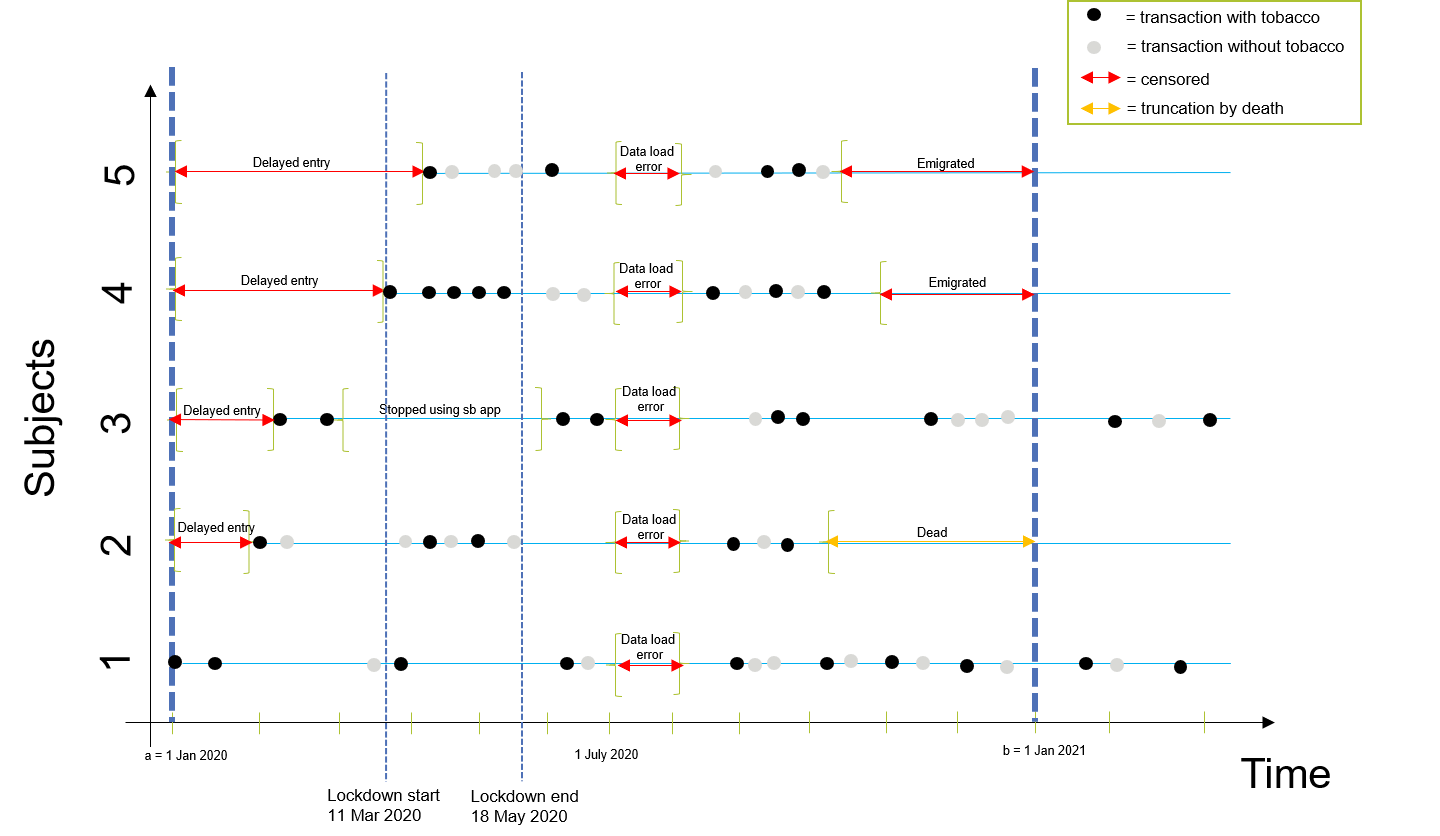
\includegraphics[]{MissingData.png}
\caption{Missing mechanisms}
\label{missing}
\end{figure}
\end{center}

Firstly, note that we have the case of truncation by death as marked by
the orange arrow. In this case, the observations are not censored, as we
know for sure that a transaction cannot happen from the grave! Secondly,
in the periods with large gap times between transactions, we do not know
whether the subject stopped using storebox, for example by changing to
another supermarket (example subject 3), or if the subject realistically
did not do frequent grocery shopping. For now we will not make any
assumptions about these transaction gap times. In the periods marked by
a red arrow, we know that the subject did not have a possibility of
making a transaction using the storebox app. Therefore, the observed
data is not complete as these periods are censored. Due to this
censoring, \(N(t)\) will not be fully observable, but only an incomplete
version, \(\tilde{N}_i(t)\) will be available for the \(i^{th}\)
subject:

\[
\tilde{N}_i(t)=N_i(t)C_i(t),
\]

where the periods with censored data are delayed entry (caused by late
entry into storebox or immigration), data load errors and emigration
(assuming that the subject does not return to Denmark in the period
\([a,b]\)). So, we define the censoring process for the \(i^{th}\)
subject as follows:

\[
C_i(t)= \begin{cases}
0 \ \ \ \text{if} \ \ a \leq t \leq \min(T_{i1}, b) \ \ \ \ \ \ \ \ \ \ \ \ \ \ \ \ \ \ \ \ \ \ \ \ \ \ \ \ \ \ \ (\text{delayed entry}) \\
0 \ \ \ \text{if} \ \ \ e1^{\text{start}} \leq t \leq \min(e1^{\text{slut}},b) \ \ \ \ \ \ \ \ \ \ \ \ \ \ \ \ \ \ \ \ \ (\text{data load error}) \\
0 \ \ \ \text{if} \ \ \ e2_i^{\text{start}} \leq t \leq \min(e2_i^{\text{slut}},b) \ \ \ \ \ \ \ \ \ \ \ \ \ \ \ \ \ \ \ \ \ (\text{emigration}) \\
1 \ \ \ \text{otherwise} \ \ \ \ \ \ \ \ \ \ \ \ \ \ \ \ \ \ \ \ \ \ \ \ \ \ \ \ \ \ \ \ \ \ \ \ \ \ \ \ \ \ \ \ \ \ \ (\text{transactions observed})
\end{cases},
\]

where \(e1_{\text{start}}, e1_{\text{slut}}\) denote the start and end
dates for a data load error (same for all subjects) and
\(e2_i^{\text{start}}, e2_i^{\text{slut}}\) denote start end dates for
emigration for subject \(i\). The censoring process is shown in Figure
\ref{censoring} for subject 2 from Figure \ref{missing}.

\begin{center}
\begin{figure}
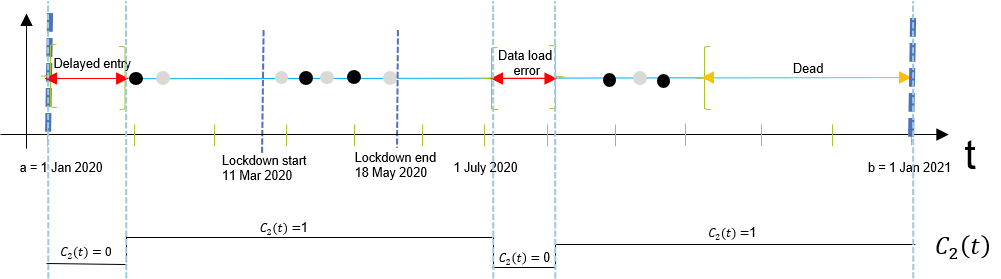
\includegraphics[]{Censoring}
\caption{Example of the censoring process $C_2(t)$ for subject 2.}
\label{censoring}
\end{figure}
\end{center}

Thus, denoting the total number of transactions for subject \(i\) by
\(K_i\), we have the following observed data for subjects \(i=1,...,n\)
in the period \([a,b]\):

\[
(C_i(t), \tilde{N}_i(t): a \leq t \leq b, \max(T_{i1},a) \leq t \leq \min(T_{iK_i},b))_{i=1}^n
\]

Our job is now to estimate a chosen target parameter based on this
observed data.

\hypertarget{estimation-of-the-target-parameter}{%
\subsection{Estimation of the target
parameter}\label{estimation-of-the-target-parameter}}

First, we write up the target parameter for tobacco for the complete
data, conditioning on information up to time \(t\). Here, we use the
tower property for conditional expectations. Let
\(N^{\text{tob}}(t)=N(t) I_{\{Q^{\text{tob}}(t) > 0, \ P^{\text{tob}}(t) > 0 \}}\)
be a counting process for tobacco transactions. We get:

\begin{align*}
\mu^{\text{tob}}(a, b) &= E(\int_a^b dN^{\text{tob}}(t))\\ 
&= E \left[ E(\int_a^b dN^{\text{tob}}(t) | \mathcal{F}_{t^-}) \right] \\
&= E \left[\int_a^b E(dN^{\text{tob}}(t) | \mathcal{F}_{t^-}) \right],
\end{align*}

We now with to estimate this target based on the intensity of buying
tobacco. From \cite{gill84} we get the definition of an
\textbf{intensity process} (here conditioning on \(\mathcal{F}_{t^-}\)):

\begin{equation}
\label{intensity}
\lambda^{\text{tob}} (t | \mathcal{F}_{t^-}) dt =P(N^{\text{tob}} \ \ \text{jumps in a time interval of length dt around time t} \ |  \mathcal{F}_{t^-})
\end{equation}

where \(\mathcal{F}_{t^-}\) (defined earlier) denotes the past up to the
beginning of the small time interval \(dt\) (everything that has
happened just before time \(t\)). In a small time interval, dt,
\(N^{\text{tob}}\) either jumps once or does not jump at all. So the
probability of a jump in that interval is close to the expected number
of jumps in that interval \cite{gill84}. From the definition of the
intensity, we therefore have:

\[
\lambda^{\text{tob}} (t|\mathcal{F}_{t^-}) dt = E(dN^{\text{tob}}(t)| \mathcal{F}_{t^-})
\]

Inserting this in the target parameter, we get:

\begin{align*}
\mu^{\text{tob}}(a, b) &= E \left[\int_a^b E(dN^{\text{tob}}(t) | \mathcal{F}_{t^-}) \right] \\
&= E \left[\int_a^b \lambda^{\text{tob}} (t|\mathcal{F}_{t^-}) dt\right]
\end{align*}

Assuming for now that expected number of tobacco transactions is
independent of tobacco shopping history and covariates, we can remove
the expectation, and thus wants to calculate (continuing the expression,
for \(i=1,...,n\) observed subjects for the interval \([a,b]\)):

\begin{align*}
\mu^{\text{tob}}(a, b) &= \int_a^b E(dN^{\text{tob}}(t))  \\
&= \sum_{i=1}^n \sum_{j \ : \ a \leq t_j \leq b} \Delta \tilde{N}_i^{\text{tob}}(t_j),
\end{align*}

where \(j=1,2,3,...\) and
\(\Delta \tilde{N}_i^{\text{tob}}(t_j)=\tilde{N}_i^{\text{tob}}(t_j)-\tilde{N}_i^{\text{tob}}(t_{j-1})\)
is the observed number of tobacco transactions for subject i between
calender day \(t_{j-1}\) and \(t_j\).

We now wish to investigate this target parameter in lockdown as compared
to the preceding period (control period). Therefore, we define the
following for the lockdown and control period:

\[
L = [11.03.2020, 18.05.2020] \ \ \text{and} \ \ \overline{L}= [02.01.2020, 10.03.2020]
\]

So, the null hypothesis that we wish to investigate is:

\[
H_0: \mu^{\text{tob}}(L)=\mu^{\text{tob}}(\overline{L})
\]

that the expected number of tobacco transactions in lockdown and the
control period is the same. In the lockdown and control period we get
the following expected number of tobacco transactions:

\[
\hat{\mu}^{\text{tob}}(L)= 1+2+5+1=9
\] \[
\hat{\mu}^{\text{tob}}(\overline{L})= 2+1+2=5
\]

Note that in order to compare these without bias, we need to make an
assumption about which subjects to include in the analysis, such that we
are comparing the same subjects in the two periods. For example, we
could choose to include only subjects who had at least one tobacco
purchase before 01-01-2020, who did not emigrate or die during any of
the two periods in order to get an unbiased, interpretable estimate.

Another way of taking the total observation time per person into account
is to model \(\hat{\lambda}^{\text{tob}}(t)\) as the tobacco transaction
rate per person-day. To estimate this based on the observed data, we
start by plugging in an estimator for the intensity, as defined in
\cite{marubini} p.~77 (again assuming constant for
\(\mathcal{F}_{t^-}\)):

\[
\hat{\lambda}^{\text{tob}}(t)=\frac{\text{total number of tobacco transactions at time t}}{\text{total observation time at time t}}
\]

So, \(\hat{\lambda}^{\text{tob}}(t)\) can be interpreted as the tobacco
transaction rate per person-day, if we consider a time unit of days.
Plugging this in and continuing the expression, for \(i=1,...,n\)
observed subjects for the interval \([a,b]\), we get (\cite{marubini}
p.~83):

\begin{align*}
\hat{\mu}^{\text{tob}}(a, b) &= \int_a^b \hat{\lambda}^{\text{tob}} (t) dt \\
&=\frac{\sum_{i=1}^n \sum_{j \ : \ a \leq t_j \leq b} \Delta \tilde{N}_i^{\text{tob}}(t_j)}{\sum_{i=1}^n \sum_{j \ : \ a \leq t_j \leq b} C_i(t_j)},
\end{align*}

where \(j=1,2,3,...\) and
\(\Delta \tilde{N}_i^{\text{tob}}(t_j)=\tilde{N}_i^{\text{tob}}(t_j)-\tilde{N}_i^{\text{tob}}(t_{j-1})\)
is the observed number of tobacco transactions for subject i between
calender day \(t_{j-1}\) and \(t_j\).

\textbf{During lockdown} for the fictive data, we get:

\begin{align*}
\hat{\mu}^{\text{tob}}(L) &= \int_L \hat{\lambda}^{\text{tob}} (t) dt \\
&=\frac{\sum_{i=1}^n \sum_{j \ : \ 11.03.20 \leq t_j \leq 18.05.20} \Delta \tilde{N}_i^{\text{tob}}(t_j)}{\sum_{i=1}^n \sum_{j \ : \  11.03.20 \leq t_j \leq 18.05.20} C_i(t_j)} \\
&=\frac{\sum_{i=1}^n \sum_{k \geq 1} I \{11.03.20 \leq T^{tob}_{ik} \leq 18.05.20\}}{\sum_{i=1}^n \sum_{j \ : \ 11.03.20 \leq t_j \leq 18.05.20} C_i(t_j)} \\
&=\frac{1+2+0+5+1}{68+68+68+68+(68-13))} \\
&=\frac{9}{327} = 0.028 \ \ \text{tobacco trans / pers-day}
\end{align*}

This gives \(0.028 \cdot 30.44 = 0.85\) tobacco transactions per
person-month in the lockdown period.

\textbf{In the control period} for the fictive data, we get (what about
death?):

\begin{align*}
\hat{\mu}^{\text{tob}}(\overline{L}) &= \int_{\overline{L}} \hat{\lambda}^{\text{tob}} (t) dt \\
&=\frac{\sum_{i=1}^n \sum_{j \ : \ 02.01.20 \leq t_j \leq 10.03.20} \Delta \tilde{N}_i^{\text{tob}}(t_j)}{\sum_{i=1}^n \sum_{j \ : \  02.01.20 \leq t_j \leq 10.03.20} C_i(t_j)} \\
&=\frac{\sum_{i=1}^n \sum_{k \geq 1} I \{02.01.20 \leq T^{tob}_{ik} \leq 10.03.20\}}{\sum_{i=1}^n \sum_{j \ : \ 02.01.20 \leq t_j \leq 10.03.20} C_i(t_j)} \\
&=\frac{2+1+2+0+0}{68+(68-30)+(68-40)+0+0} \\
&=\frac{5}{134}=0.037 \ \ \text{tobacco trans / pers-day}
\end{align*}

See Figure \ref{missing} to see the censored periods subtracted from the
person-days in the denominator.

This gives \(0.023 \cdot 30.44 = 1.13\) tobacco transactions per
person-month in the control period.

\newpage

\begin{itemize}
\tightlist
\item
  Consider to include the following points in the introduction:
\item
  Data from hospital records (s. 9 uk inequelities)
\item
  Lack of large sample sizes to be able to include confounders
  (spotlight).
\item
  Differences at community level, not changes in specific participants'
  behaviour (p.~7 california).
\item
  Research wise, an interesting perspective is that this turns an
  observational study into an interventional study.
\item
  Stockpiling behaviour (letter).
\item
  Not random sample (california), like in our case. Impacts
  generalizability. (p.~7)
\item
  Impact on smoking cessation messages
  (\url{https://www.ncbi.nlm.nih.gov/pmc/articles/PMC8083603/})
\end{itemize}

\newpage 
\begin{thebibliography}{1}

\bibitem{fda} FDA. (2020, April 5). How Smoking Affects Heart Health. Health Effects of Tobacco Use. https://www.fda.gov/tobacco-products/health-effects-tobacco-use/how-smoking-affects-heart-health.

\bibitem{sundhedsstyrelsen} Sundhedsstyrelsen. (2018, March 6). Danskernes Sundhed - Den Nationale Sundhedsprofil 2017. https://www.sst.dk/da/udgivelser/2018/danskernes-sundhed-den-nationale-sundhedsprofil-2017

\bibitem{turkish} Tetik, B. K., Tekinemre, I. G., Tas, S. (2021, June). \textit{The Effect of the Covid-19 Pandemic on Smoking Cessation Success.}. Journal of Community Health. 46(3):471-475. doi: 10.1007/s10900-020-00880-2.

\bibitem{wave3} Gravely, S., Craig, L. V., Cummings, K. M. et al. (2021, June 04). \textit{Smokers' cognitive and behavioural reactions during the early phase of the COVID-19 pandemic: Findings from the 2020 ITC Four Country Smoking and Vaping Survey}. Plos One. 16(6):e0252427. doi: 10.1371/journal.pone.0252427.

\bibitem{unionbrief} International Union Against Tuberculosis and Lung Disease (2021, August 17). \textit{COVID-19 and TOBACCO: THE UNION’S BRIEF (Final Update: 17 August 2021)}. https://theunion.org/our-work/covid-19/covid-19-and-smoking.

\bibitem{todolist} Algatani, J. S., Aldhadir, A. M., Oyelade, T. et al. (2021, May 06). \textit{Smoking cessation during COVID-19: the top to-do list}. NPJ Primary Care Respiratory Medicine. 31: 22. doi: 10.1038/s41533-021-00238-8.

\bibitem{addiction} Jackson, E. J., Garnett, C., Shahab, L. et al. (2021, May). \textit{Association of the COVID-19 lockdown with smoking, drinking and attempts to quit in England: an analysis of 2019-20 data}. Addiction. 116(5):1233-1244. doi: 10.1111/add.15295.

\bibitem{california} Gonzalez, Epperson, A. E., Halpern-Felsher, B. et al. (2021, March 05). \textit{Smokers Are More Likely to Smoke More after the COVID-19 California Lockdown Order}. Int J Environ Res Public Health. 18(5): 2582. doi: 10.3390/ijerph18052582.

\bibitem{UK_inequalities} Jackson, E. J, Brown, J., Shahab, L., Steptoe, A., Fancourt, D. et al. (2020, August 21). \textit{COVID-19, smoking and inequalities: a study of 53 002 adults in the UK}. Tobacco Control. doi: 10.1136/tobaccocontrol-2020-055933.

\bibitem{digital} El-Toukhy, S. (2021, March 22). \textit{Insights From the SmokeFree.gov Initiative Regarding the Use of Smoking Cessation Digital Platforms During the COVID-19 Pandemic: Cross-sectional Trends Analysis Study}. Journal of medical internet research. doi: 10.2196/24593.

\bibitem{gill82} Gill, D. R., Andersen, P. K. (1982). \textit{Understanding Cox's Regression Model: A Martingale Approach}, The Annals of Statistics, 10 (4), p. 1100-1120.

\bibitem{gill84} Gill, D. R. (1984). \textit{Understanding Cox's Regression Model: A Martingale Approach}, Journal of the American Statistical Association, 79 (386), p. 441-447.

\bibitem{statlearning} Hastie, T., Tibshirani, R., Friedman, J. (2009). \textit{The Elements of Statistical Learning} (Second ed.). Springer. 

\bibitem{kar} Karr, A. F. (1986). \textit{Point Processes and Their Statistical Inference} (First Ed.). Marcel Dekker.

\bibitem{last} Last, G., Brandt, A. (1995). \textit{Marked Point Processes on the Real Line} (First Ed.). Springer.

\bibitem{marubini} Marubini, E. (1995). \textit{Analysing Survival Data from Clinical Trials and Observational Studies} (First Ed.). John Wiley and Sons.

\bibitem{pis} Pishro-Nik, H. (2014). \textit{Introduction to Probability, Statistics, and Random Processes} (First ed.). Kappa Research. 

\bibitem{ch5} Tan, P. N., Steinbach, M., Karpatne, A., Kumar, V. (2019). \textit{Introduction to Data Mining} (First ed.). Pearson.

\bibitem{bay} Walley, Rosalind et al. (2016). \textit{Using Bayesian analysis in repeated preclinical in vivo studies for a more effective use of animals}, Pharmaceutical Statistics, No. 15, 2016, p. 277-285.

\end{thebibliography}

\end{document}
